\documentclass[12pt, preprint]{aastex}

\usepackage{subfigure}
\usepackage{color}
\usepackage{hyperref}
\usepackage{url}
\usepackage{natbib}

\newcommand{\project}[1]{\textsl{#1}} 
\newcommand{\galex}{\project{GALEX}}
\newcommand{\cause}{\project{GALEX CAUSE}}
\newcommand{\scanmode}{\project{scan-mode}}
\newcommand{\gphoton}{\project{gPhoton}}
\newcommand{\todo}[1]{\textbf{#1}}

\bibliographystyle{apj}
\definecolor{linkcolor}{rgb}{0,0,0.5}
\hypersetup{colorlinks=true,linkcolor=linkcolor,citecolor=linkcolor,
            filecolor=linkcolor,urlcolor=linkcolor}

\begin{document}

\title{\galex\ \scanmode\ Data}
\author{}

\section{Description of Data}
The Galaxy Evolution Explorer (\galex, \citealt{galex}) is a space-based telescope investigating the causes and evolution of star formation in galaxies in UV band.

After the original \galex\ was finished, the mission was extend to the \cause\ phase, in which the telescope was operated in a mode know as \scanmode.
In contrast to the traditional boresight dither, the telescope traverses around the galactic plane rapidly. 
The \scanmode\ enables the team to  complete the All-Sky UV Survey in a short time and avoid saturation caused by the high stellar density in the survey region.

Data used in this project are the raw photon data(-raw6.fits), the refined attitude solution (-asprta.fits), and the spacecraft state file (-scst.fits). This project also heavily depend on the photon list produced by \gphoton (\url{https://github.com/cmillion/gPhoton}), in which each photon event is tagged with position  and time.

\section{Calibration}

\subsection{Freedom of the telescope}


\subsection{Cross-correlation of photons and star catalog}
To characterize the offsets of the pointing and the rotation correction of the detector, the cross-correlation of photons and star catalog are calculated. 

\begin{figure}[p]
\begin{center}
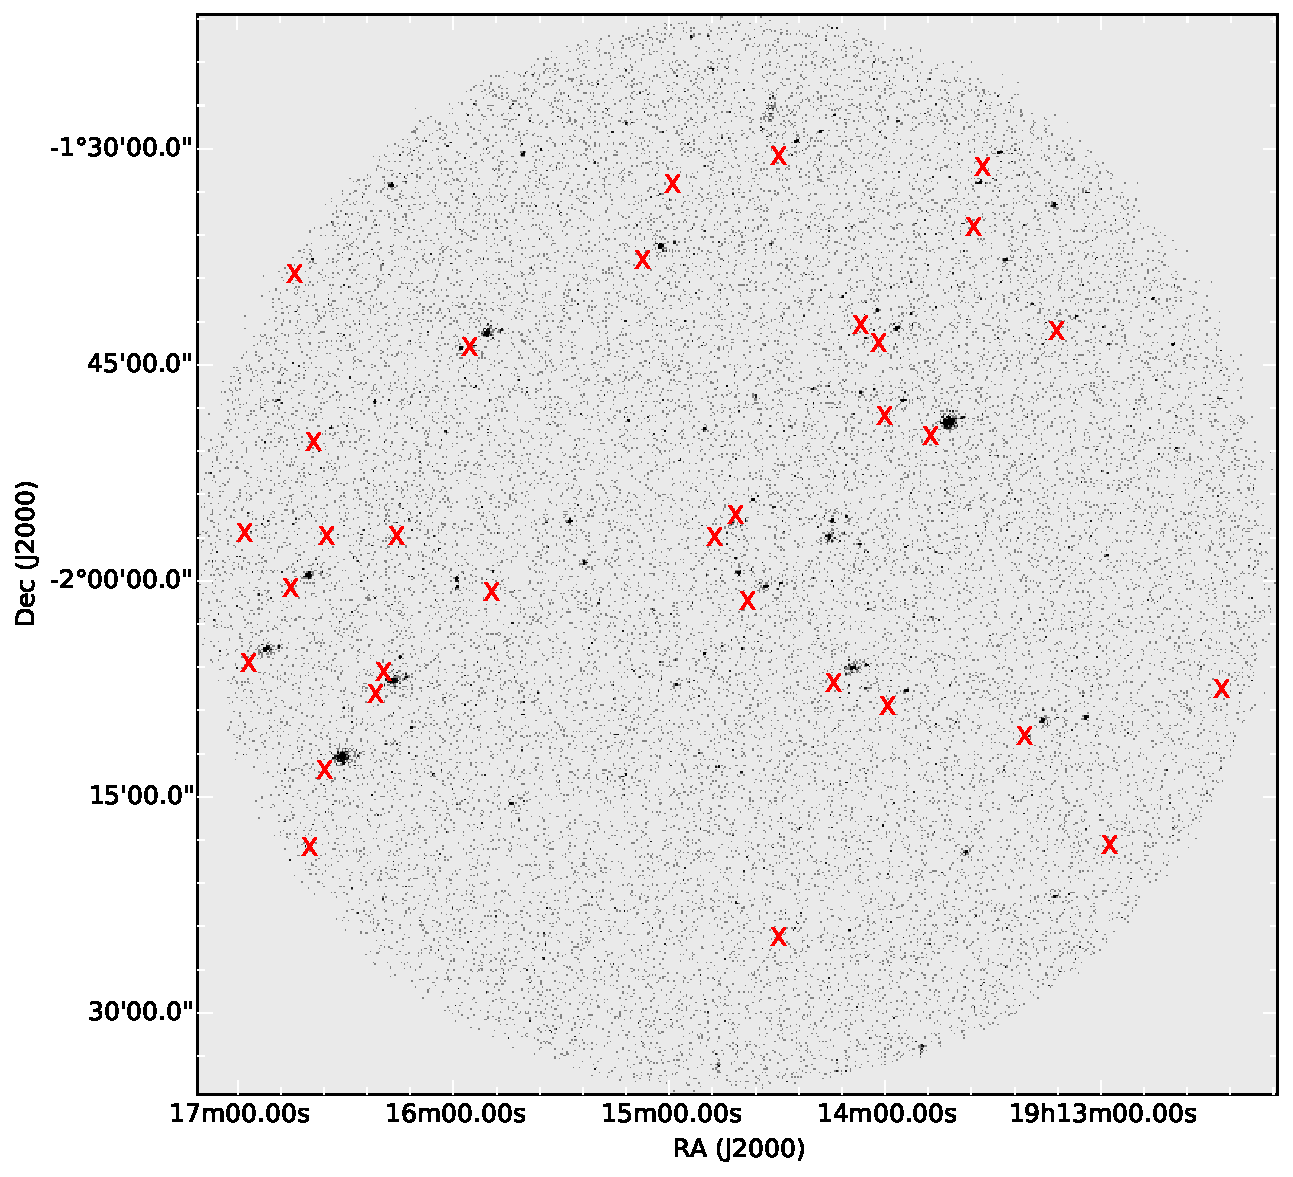
\includegraphics[width=0.6\textwidth]{figures/slice.pdf}
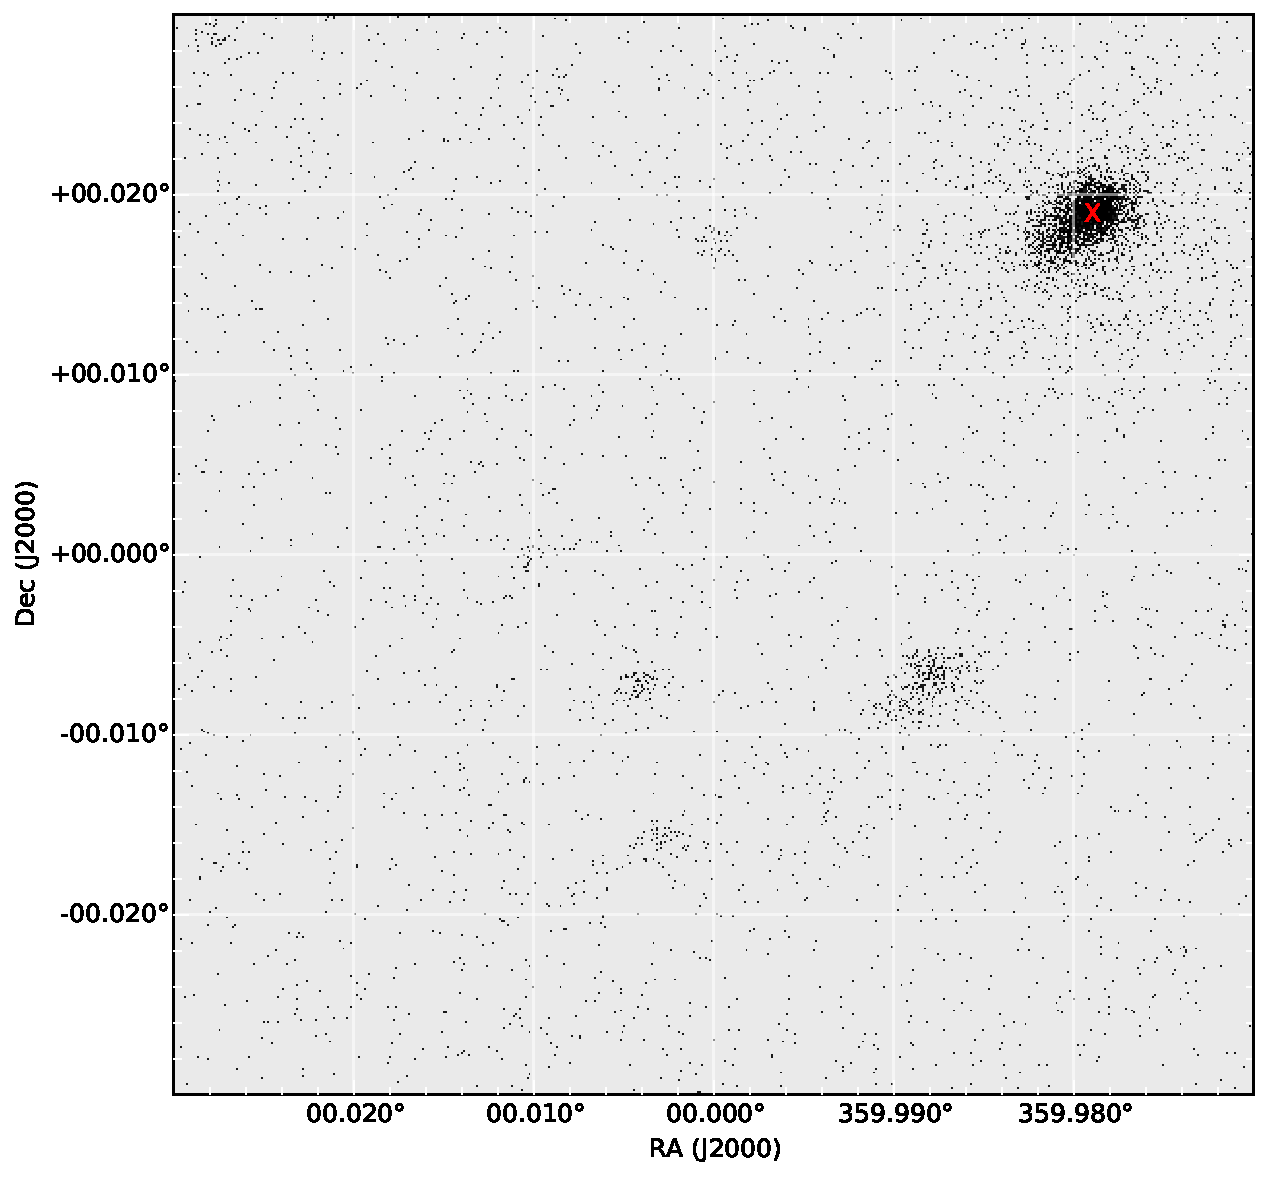
\includegraphics[width=0.6\textwidth]{figures/corr.pdf}
\end{center}
\caption{%
  \label{slice}
  Cross-correlation of photons and star catalog.
  \emph{Top:}  An one second snapshot of the photons on the sky. The black points are the location of the photons. The red crosses indicate the location of the stars from the input catalog. It is quite obvious that there is a small offset between photons and the stars.
  \emph{Bottom:} The cross-correlation of photons and stars. Each black points in the plot shows a pair of photon and star that have a certain displacement. The red cross indicates the centroid of the cross-correlation fucntion, which is the overall offsets between photons and stars---the offset of the pointing.
  }
\end{figure}


\section{Sky map construction}
\subsection{Count map}
To construct the sky map image, the photon list (list of photons tagged with position and time) should be binned into pixels. In this project, the pixel size is 1.5 arcsec. The count map is defined as the binned photon image as shown in the upper panel of Fig.~\ref{map}
 
\subsection{Exposure map}
The exposure map is the defined as the following integral:
\begin{eqnarray}
  exposure &=& \int_{t_0}^{t_1}f(1-D)dt
\end{eqnarray}
where f is the flat-field, D is the dead time recorded in the spacecraft state file (-scst.fits). The lower and upper limit of the integral $t_0$, $t_1$ are the beginning and ending time of the scan.

\subsection{Intensity map}
After the count map and exposure map are constructed, the intensity map is defined as the ratio these two maps:
\begin{eqnarray}
  intensity &=& \frac{count}{exposure}
\end{eqnarray}

\begin{figure}[p]
\begin{center}
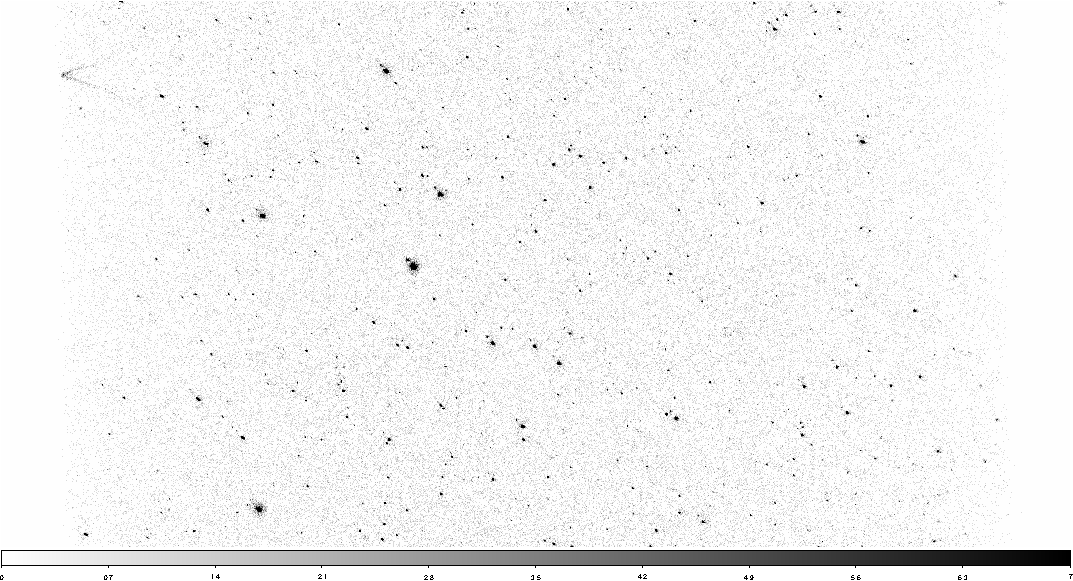
\includegraphics[width=0.6\textwidth]{figures/count.pdf}
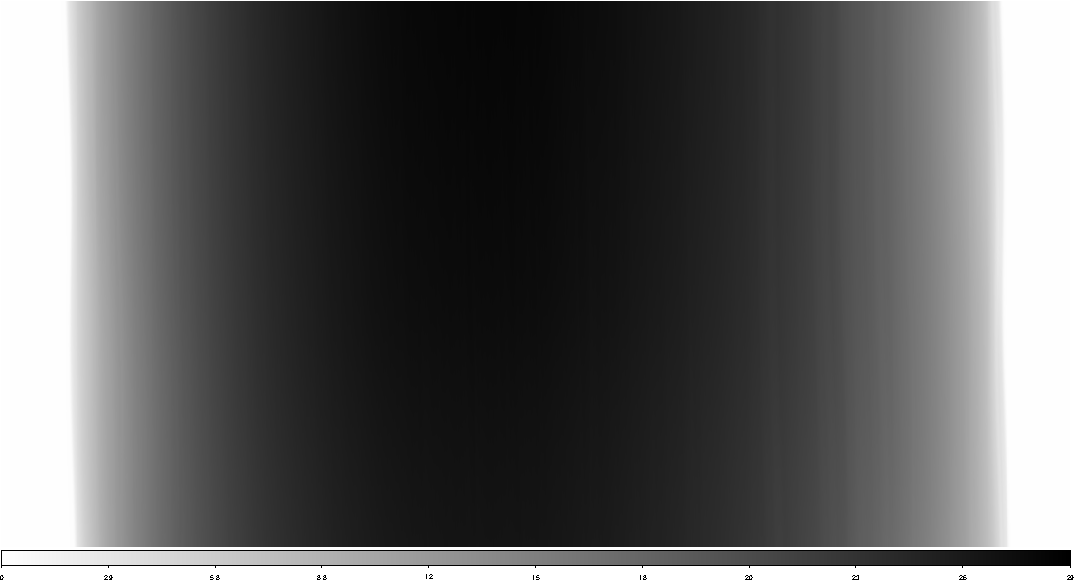
\includegraphics[width=0.6\textwidth]{figures/exp.pdf}
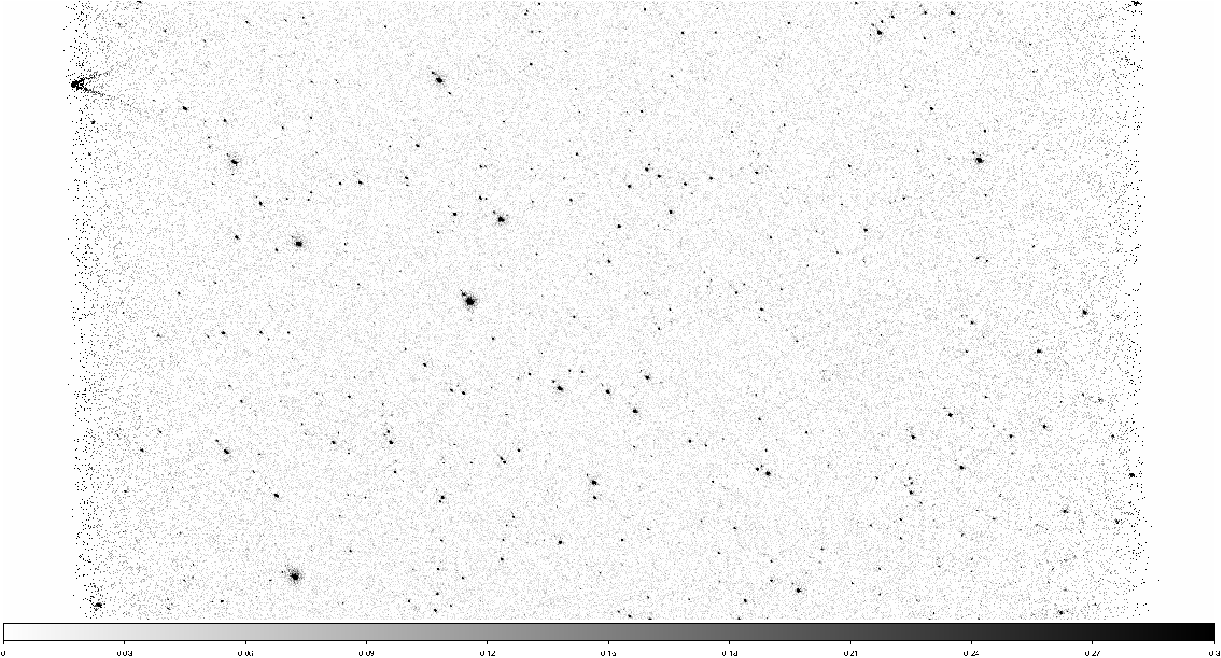
\includegraphics[width=0.6\textwidth]{figures/intensity.pdf}
\end{center}
\caption{%
  \label{map}
  Example images of \galex\ \scanmode\ data.
  The top panel is the count map of the region($288.79\ deg<gl<290.50\ deg, 7.74\ deg<gb<8.43\ deg$). 
  The image grows faint in both edges, since the exposure time is lower on the edges.
  The middle panel shows the exposure map in the same reigon of the count map from the top panel.
  The bottom panel is the intensity map calculated from the top two images. 
  It clearly shows correction of the exposure especially on the edges.
  }
\end{figure}

\section{Source Extraction}
Once the images were constructed, we used SExtractor (\cite{sextractor}) to detect sources and measure their positions and fluxes (using the FLUX\_AUTO parameter). We used a modified version of the default input SExtractor configuration with the goal of minimizing false detections at the edges of the images. We found that the background subtraction step in SExtractor introduced an artificial level of noise from the image edges. To avoid this issue altogether we cut the image into a subsection that removed the outer scan edges and then ran SExtractor. We then converted the fluxes to GALEX NUV AB magnitudes using NUV = -2.5 * log10(FLUX) + 20.08.

The scan data had overlaps of about .25 degrees on each side, producing duplicates in the SExtractor output. To deal with this issue we looked at the overlapping regions and compared their coordinates between scans and flagged any matches. Finally, we only used SExtractor data from the sources that had the highest signal to noise.

To test the accuracy of our NUV measurements, we compared our measurements with the GALEX All Sky Imaging Survey which included regions in the Galactic plane. We gathered 16,851,560 objects within the same limits as the GALEX Plane Survey (360$\deg$ x 20$\deg$ from abs(gb) $<$ 10). The magnitudes agree very well from 14 $<$ m$_{NUV}$ $<$ 18. 

\begin{table}
\begin{tabular}{cc}
DETECT\_TYPE & CCD \\
DETECT\_IMAGE & SAME \\
FLAG\_IMAGE & flag.fits \\
DETECT\_MINAREA & 8 \\
DETECT\_THRESH & 2.5 \\
ANALYSIS\_THRESH & 2 \\
FILTER & Y \\
FILTER\_NAME & default.conv \\
DEBLEND\_NTHRESH & 32 \\
DEBLEND\_MINCONT & 0.005 \\
CLEAN & Y \\
CLEAN\_PARAM & 1.0 \\
BLANK & Y \\
PHOT\_APERTURES & 10 \\
PHOT\_AUTOPARAMS & 2.5,  3.5 \\
SATUR\_LEVEL & 50000.0 \\
MAG\_ZEROPOINT & 0.0 \\
MAG\_GAMMA & 4.0 \\
GAIN & 100.0 \\
PIXEL\_SCALE & 7.2 \\
BACK\_SIZE & 64 \\
BACK\_FILTERSIZE & 3 \\
BACKPHOTO\_TYPE & GLOBAL \\
BACKPHOTO\_THICK & 24 \\
CHECKIMAGE\_TYPE & BACKGROUND \\
MEMORY\_OBJSTACK & 2000 \\
MEMORY\_PIXSTACK & 100000 \\
MEMORY\_BUFSIZE & 512 \\
SCAN\_ISOAPRATIO & 0.6 \\
VERBOSE\_TYPE & NORMAL \\
\end{tabular}
\end{table}

\clearpage
\bibliography{gs}
\clearpage

\end{document}
